\documentclass[dvipdfmx,autodetect-engine,titlepage]{jsarticle}
\usepackage[dvipdfm]{graphicx}
\usepackage{ascmac}
\usepackage{fancybox}
\usepackage{listings}
\usepackage{plistings}
\usepackage{itembkbx}
\usepackage{amsmath}
\usepackage{url}
\usepackage{graphics}
\usepackage{listings}
\usepackage{here}

\lstset{%
  language={C},
  basicstyle={\small},%
  identifierstyle={\small},%
  commentstyle={\small\itshape\color[rgb]{0,0.5,0}},%
  keywordstyle={\small\bfseries\color[rgb]{0,0,1}},%
  ndkeywordstyle={\small},%
  stringstyle={\small\ttfamily\color[rgb]{1,0,1}},
  frame={tb},
  breaklines=true,
  columns=[l]{fullflexible},%
  numbers=left,%
  xrightmargin=0zw,%
  xleftmargin=3zw,%
  numberstyle={\scriptsize},%
  stepnumber=1,
  numbersep=1zw,%
  lineskip=-0.5ex%
}

\textheight=23cm
\renewcommand{\figurename}{図}
\renewcommand{\tablename}{表}
\newenvironment{code}
{\vspace{0.5zw}\VerbatimEnvironment  \begin{screen} 
\baselineskip=1.0\normalbaselineskip
 \begin{Verbatim}}
{\end{Verbatim}
\baselineskip=\normalbaselineskip
 \end{screen}\vspace{0.5zw}} 

\title{自然言語処理(R)\\
第7回レポート\\
}
\author{26002000872\\Oku Wakana\\奥 若菜}
\date{Jun. 2 2022}

\begin{document}

\maketitle

\section{課題内容}
与えられた日本語文法を用いて「ヒロシが病院でもらった薬を飲んだ」という文章を上昇型チャート法で解析し、その流れを示す。\\\\

\section{上昇型チャート法による解析}
与えられた文章を上昇型チャート法で解析し、下の表1に流れを示した。\\

 \begin{table}[H]
    \centering
    \caption{解析表}\label{fig:表}
    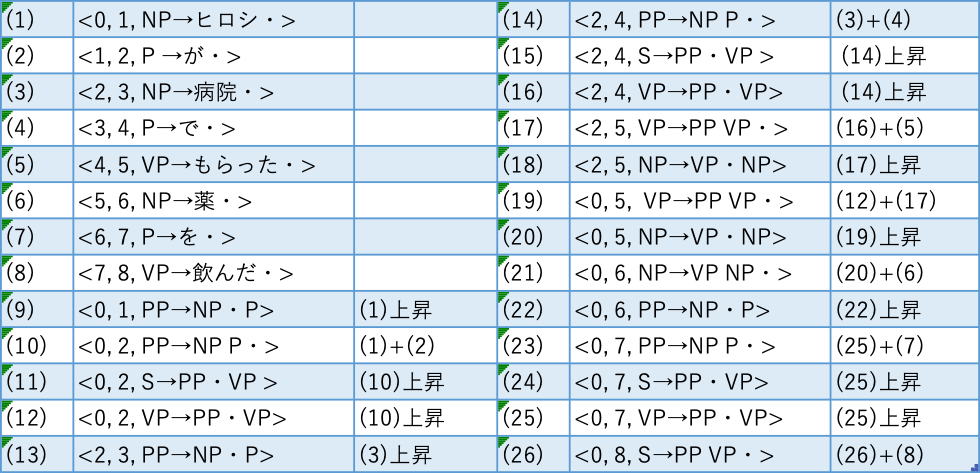
\includegraphics[scale=0.3]{fg1.png}
\end{table}

\section{結果}
表1から作成した構文木が下の図1である。\\

 \begin{figure}[H]
    \centering
    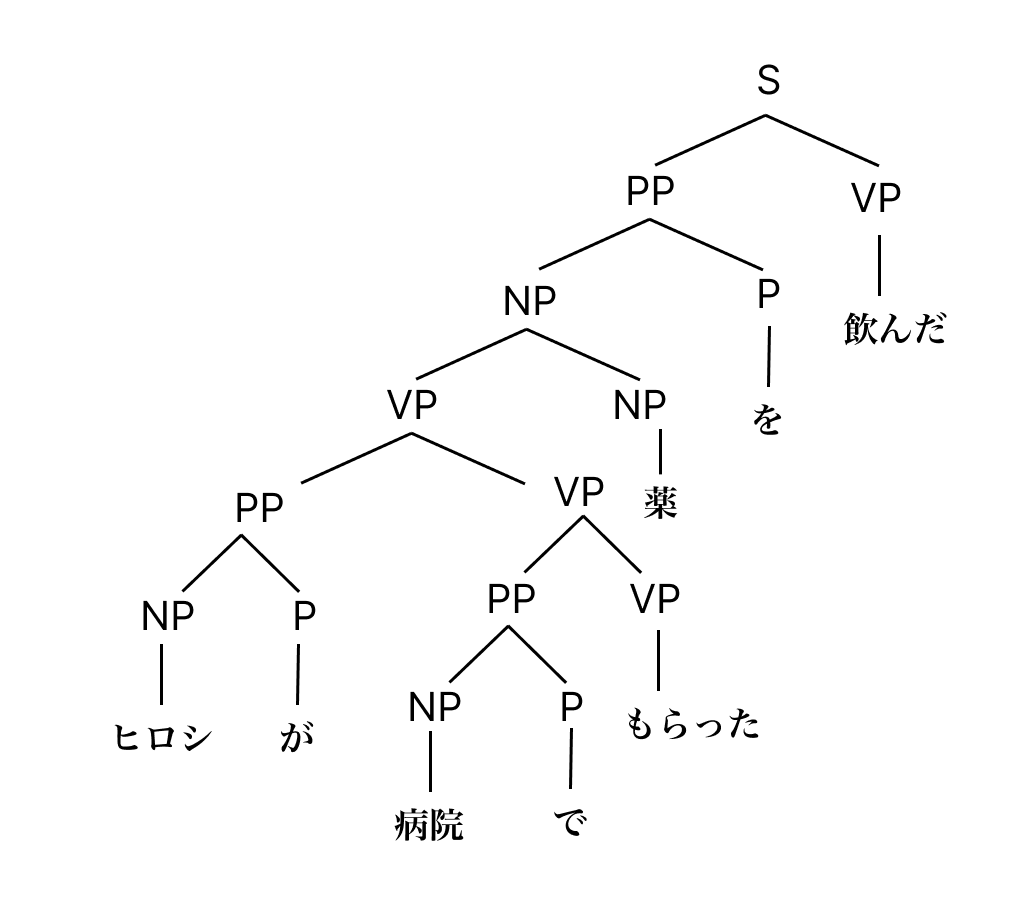
\includegraphics[scale=0.17]{tree1.png}
    \caption{構文木}\label{fig:図}
\end{figure}


\end{document}